% !TEX spellcheck = en_US
% !TeX root = Lecture.tex
%---------------------------------------------------------------------------------
\section[Airfoil Aerodynamics]{Airfoil Aerodynamics}\label{sec:AAD}
%---------------------------------------------------------------------------------
\miniframesoff
\begin{frame}<handout:0>[noframenumbering]{Content}
\tableofcontents[currentsection]
\PutAt<1-|handout:0>[5cm]{(10cm,2cm)}{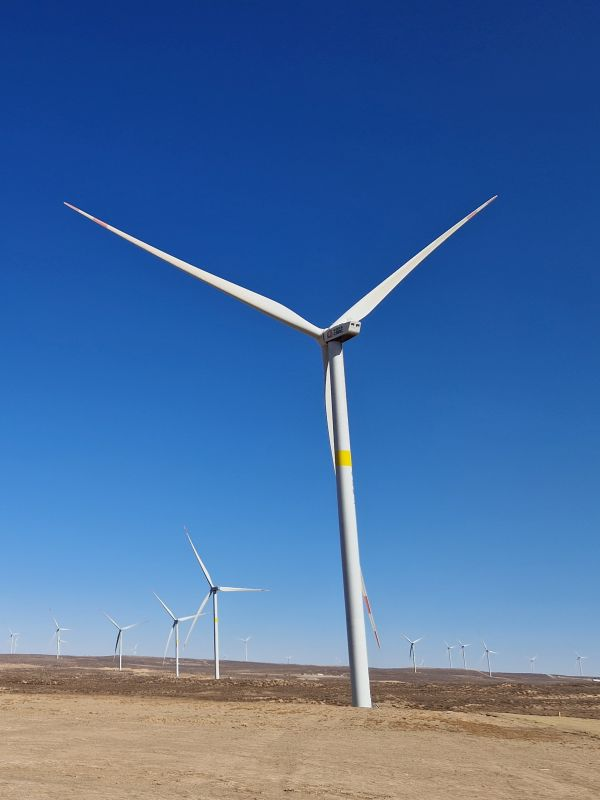
\includegraphics[width=4.0cm]{\StylePath/content/Gobi}} % graphic related to topic	
\end{frame}
\miniframeson
%---------------------------------------------------------------------------------
\begin{frame}{Airfoil} 
\begin{columns}
	\column{7cm}
		\centering
		\includegraphics<1->[width=7.0cm] {AAD/Airfoil}\\
		{\tiny\textcolor{gray}{[\href{https://en.wikipedia.org/wiki/Airfoil}{wikipedia}]}}		
	\column{7cm}
		\begin{block}<1->{Definition}
		 	\begin{itemize}
				\item In fluid dynamics an airfoil is referred to as the shape of a solid bodies cross-section in flow direction.
				\item Due to the specific shape of the airfoil, a flow of a fluid or a gas will generate external forces on the body.
			\end{itemize}						 
		\end{block}
\end{columns} 	
\end{frame}
%---------------------------------------------------------------------------------
\begin{frame}{Simplified Physical Explanations of Lift on an Airfoil 1/3} 
\begin{columns}
	\column{6cm}
		\centering
		\includegraphics<1->[width=6.0cm] {AAD/AirfoilDeflectionLift_W3C}\\
		{\tiny\textcolor{gray}{[\href{https://en.wikipedia.org/wiki/Lift_(force)}{wikipedia}]}}				
	\column{8cm}
		\begin{block}<1->{Flow deflection and Newton's laws}	
		 	\begin{itemize}
				\item As the air flow passes the airfoil, it changes the direction downwards.
				\item According to Newton's 2nd law (``$F=ma$'') this requires a downward force, which is applied to the air by the airfoil.
				\item According to Newton's 3rd law (``action-reaction-law'') a reaction force is applied to the airfoil by the air, which pushes the airfoil upwards.
			\end{itemize}				
		\end{block}
\end{columns} 	
\end{frame}
%---------------------------------------------------------------------------------
\begin{frame}{Simplified Physical Explanations of Lift on an Airfoil 2/3} 
\begin{columns}
	\column{6cm}
		\centering
%		\includegraphics<1->[width=6.0cm] {AAD/Karman_trefftz.png}\\
		\animategraphics[loop,autoplay,width=6cm]{30}{AAD/Karman_trefftz_gif/Karman_trefftz-}{0}{79}
		{\tiny\textcolor{gray}{[\href{https://en.wikipedia.org/wiki/Lift_(force)}{wikipedia}]}}
	\column{8cm}
		\begin{block}<1->{Increased flow speed and Bernoulli's principle}	
			\begin{itemize}
			    \item The streamlines on the upper side of the airfoil are compressed, so the flow speed is increased.
				\item The velocity of the air on the upper side of the airfoil is higher  than on the lower side.
				\item Due to Bernoulli's law increased speed causes an area with lower pressure (suction side) and decreased speed causes an area with higher pressure (pressure side).
				\item This difference in pressure generates a force acting from the pressure side towards the suction side of the airfoil.
			\end{itemize}			
		\end{block}
\end{columns} 	
\end{frame}
%---------------------------------------------------------------------------------
\begin{frame}{Simplified Physical Explanations of Lift on an Airfoil 3/3} 
\centering
\includegraphics<1->[height=7.0cm] {AAD/UnderstandingAerodynamicLift}\\
{\tiny\textcolor{gray}{[\href{https://www.youtube.com/watch?v=E3i_XHlVCeU}{youtube - The Efficient Engineer}]}}					
\end{frame}
%---------------------------------------------------------------------------------
\begin{frame}{How do Wings Work?} 
\begin{columns}
	\column{4.5cm}
	\centering
	\includegraphics<1->[height=7.2cm] {AAD/Babinsky2003_Fig7_to_9}
	\column{9.5cm}
	\begin{block}<1->{Another explication \cite{Babinsky2003}}	
		\begin{itemize}
			\item A particle on a curved streamline is changing direction. Therefore a centripetal force must exist. This accelerating force is generated by pressure differences (pressure gradient perpendicular to the streamline).
			\item The pressure is decreasing towards the center of curvature. In A and C the pressure is equal ($p_{\textnormal{A}}=p_{\textnormal{C}}=p_{\textnormal{atm}}$). Going on a line from A to B the pressure decreases towards B ($p_{\textnormal{A}}>p_{\textnormal{B}}$). Going on a line from C to D the pressure increases towards D ($p_{\textnormal{C}}<p_{\textnormal{D}}$).
			\item This means $p_{\textnormal{B}}<p_{\textnormal{D}}$. The pressure difference will generate lift.
			\item  \href{https://www.cam.ac.uk/research/news/how-wings-really-work}{[Video University of Cambridge]}
		\end{itemize}			
	\end{block}
\end{columns} 			
\end{frame}
%---------------------------------------------------------------------------------
\begin{frame}{Solution to the Problem} 
\begin{columns}
	\column{8.5cm}
	\centering
	\includegraphics<1->[width=8.5cm] {AAD/Ansys}\\
	{\tiny\textcolor{gray}{[\href{https://www.youtube.com/watch?v=ngNZdyWTUIo}{youtube - ANSYS CFX Tutorial}]}}	
	\column{5.5cm}
	\begin{block}<1->{More complex solution}	
		 Calculate lift via CFD using 
		\begin{itemize}
			\item Conservation of momentum
			\item Conservation of mass
			\item Conservation of energy
		\end{itemize}			
	\end{block}
	\begin{block}<2->{Simple solution}	
		\begin{itemize}
			\item Experts still discuss about a simplified physical explanation
			\item Important for us: flow over an airfoil generates lift and drag!
		\end{itemize}			
	\end{block}
\end{columns} 			
\end{frame}
%---------------------------------------------------------------------------------
\begin{frame}{Lift and Drag} 
\setlength{\abovedisplayskip}{0pt}
\setlength{\belowdisplayskip}{1pt}
\begin{columns}	
	\column{7cm}
	\begin{block}<1->{Lift force $L$ and drag force $D$}
		\begin{align*}
		L   & = \frac{1}{2} \rho \left(cb\right) c_{\textnormal{L}}(\alpha_{\textnormal{A}}) w^2\\
		D   & = \frac{1}{2} \rho \left(cb\right) c_{\textnormal{D}}(\alpha_{\textnormal{A}}) w^2
		\end{align*}
		\begin{tabular}{ll}
			$c_{\textnormal{L}}$ 		&  	lift coefficient\\
			$c_{\textnormal{D}}$ 		&  	drag coefficient\\
			$\alpha_{\textnormal{A}}$ 	&  	angle of attack\\
			$c$ 					& 	chord length \\
			$b$ 					& 	chord width \\
			$w$ 					& 	local (relative) wind velocity
		\end{tabular}	
	\end{block}
	\column{7cm}
	\centering
	\includegraphics<1->[width=7.0cm] {AAD/LiftAndDrag.pdf}
	\begin{block}{Per definition}
		\begin{itemize}
			\item Lift perpendicular to $w$
			\item Drag parallel to $w$	
		\end{itemize}
	\end{block}
\end{columns} 	
\end{frame}
%---------------------------------------------------------------------------------
\begin{frame}{Example: NACA64 A17 of NREL 5~MW RWT} 
\begin{columns}	
	\column{7cm}
	\centering
	\includegraphics<1->[height=3.5cm] {AAD/NREL5MW}\\
	{\tiny\textcolor{gray}{\cite{Jonkman2009a}}}
	\begin{block}{Reference Wind Turbine}
		\begin{itemize}
			\item for FAST (open source)
			\item $\SI{126}{\meter}$ rotor diameter
			\item $\SI{90}{\meter}$ hub height
			\item NACA64 for tip region		
		\end{itemize}
	\end{block}	
	\column{7cm}
	\includegraphics<2->[width=7.cm] {AAD/NACA64_618}\\
	\includegraphics<2->[width=7.cm] {AAD/NACA64_LiftAndDrag}
\end{columns} 	
\end{frame}
%---------------------------------------------------------------------------------
\begin{frame}[t]{Lift-To-Drag Ratio} 
\setlength{\abovedisplayskip}{0pt}
\setlength{\belowdisplayskip}{1pt}
\vspace{-6pt}% to avoid overfull vbox
\begin{columns}[T]
	\column{7cm}
	\begin{block}<1->{Lift-to-drag (L2D) ratio $\varepsilon$}
		\begin{align*}
		\varepsilon(\alpha_{\textnormal{A}})   & = \frac{c_{\textnormal{L}}(\alpha_{\textnormal{A}})}{c_{\textnormal{D}}(\alpha_{\textnormal{A}})} 
		\end{align*}
		\begin{tabular}{ll}
			$c_{\textnormal{L}}$ 		&  	lift coefficient\\
			$c_{\textnormal{D}}$ 		&  	drag coefficient\\
			$\alpha_{\textnormal{A}}$ 	&  	angle of attack\\
		\end{tabular}\\
		\begin{itemize}
			\item max $\varepsilon$ is a measure for airfoil quality
			\item simple board up to $\varepsilon\approx10$ 
			\item<2-> equal to L2D ratio for airplanes		
			\item<3-> $\alpha_{\textnormal{A}}$ at which $\varepsilon$ reaches its maximum can be found by tangent on Lilienthal polars
		\end{itemize}		
	\end{block}	
	\centering
	\includegraphics<2->[width=4.0cm] {AAD/Gleitzahl}
	\visible<2->{\tiny\textcolor{gray}{[www.mgow.ch]}}
	\column{7cm}
	\includegraphics<1->[width=7.cm] {AAD/NACA64_LiftToDrag}\\
	\includegraphics<3->[width=7.cm] {AAD/NACA64_Lilienthal}
\end{columns} 	
\end{frame}
